\documentclass{article}
\usepackage[english]{babel}
\usepackage[letterpaper,top=2cm,bottom=2cm,left=3cm,right=3cm,marginparwidth=1.75cm]{geometry}
\usepackage{amsmath}
\usepackage{graphicx}
\usepackage{listings}
\usepackage{physics}
\usepackage{caption}
\usepackage{titlesec}
\usepackage[dvipsnames]{xcolor}
\usepackage[colorlinks=true, allcolors=blue]{hyperref}
\usepackage{pdfpages}

\usepackage{tikz}
\usepackage{pgfplots}
\pgfplotsset{compat=1.18}

\lstdefinestyle{python_style}{
    backgroundcolor=\color{white},
    tabsize=4,
    basicstyle=\footnotesize\ttfamily,
    language=Python,
    captionpos=b,
    tabsize=3,
    frame=lines,
    numbers=left,
    numberstyle=\tiny,
    numbersep=5pt,
    breaklines=true,
    showstringspaces=false,
    keywordstyle=\color{blue},
    commentstyle=\color{OliveGreen},
    stringstyle=\color{red}
}

\begin{document}

\begin{figure}[h!]
    \centering
    \includegraphics[width=0.64\textwidth]{graphics/UScrest-top-eps-converted-to.pdf}\par\vspace{1cm}
    {\scshape\Large Movie Recommender System using Matrix Factorization\par}
    \vspace{0.75cm}
    {\Large Lucas Meyer\par}
    \vspace{0.05cm}
    {\normalsize \href{22614524@sun.ac.za}{22614524@sun.ac.za}\par}
    \vspace{0.05cm}
    {\normalsize \today\par}
    \vspace{0.7cm}
\end{figure}

\abstract{
    This report is a summary of the work that I have done for a MSc course called ``Applied Machine Learning at Scale''.
    The course is coordinated by Ulrich Paquet~\cite{Ula} and is presented at the University of Stellenbosch.
    The main output of the course is to program a recommender system for movies, using the MovieLens dataset.
    This report is an explanation of the movie recommender system that I have implemented throughout the duration of the course.
}

\section{Introduction}
In recent years, recommender systems have gained significant importance in various applications
such as e-commerce, social networking, and personalized marketing. Typically, recommender systems assist
users in making choices by providing them with personalized recommendations based on their past
behavior, preferences, and feedback. In the case of streaming sevices such as Netflix (movies and series), 
the use of a recommender system may improve user satisfaction and, as a result of this, convince users to
continue using the service.

In this report, I present an implementation of a movie recommender system using Yehuda's matrix
factorization method~\cite{Yehuda}. The results of the recommender system is based on 
the MovieLens dataset~\cite{MovieLens}. The MovieLens dataset is a commonly used benchmark
dataset in the field of recommender systems that contains a collection of user ratings of movies, and genre
information relating to each movie in the dataset.

The recommender system discussed in this report utilizes explicit data (user ratings).
In contrast, implicit data is observed user behavior such as clicks or purchases (without the explicit rating).
The main difference between explicit and implicit movie data is that explicit data may provide more accurate information
about user preferences, while implicit data relies on assumptions about user behaviour\footnote{Implicit feedback is not utilized in this report. 
For those interested, Steffen et al. proposed recommender system that utilizes implicit feedback to make predictions using 
Bayesian analytics~\cite{BPR}.}.

The layout of the report is as follows. A description of the MovieLens data and statistical analysis of the dataset(s)
is given in Section 2. The matrix factorization method is explained in detail throughout Section 3.
The evaluation techniques are briefly discussed in Section 4, and parameter tuning is discussed in Section 5.
Section 6 is a summary of several different experimental results, and Section 7 concludes this report with
a discussion of the advantages and disadvantages of the recommender system, along with a brief discussion of future work.

\newpage

\section{Datasets}

\subsection{Description of the MovieLens Datasets}
There are many versions of the MovieLens dataset.
Each version of the MovieLens dataset contains a collection of movie ratings that range from 0.5 to 5, with increments of 0.5.
The datasets also provide additional metadata about the movies (title, year of release, and genre).
There are two MovieLens datasets that are used in this report:

\begin{enumerate}
\item \textbf{Latest-small dataset:} This dataset contains $100,000$ ratings from $610$ different users for $9724$ unique movies.
This dataset is a subset of the full MovieLens dataset and is commonly used for quick
experimentation and prototyping of recommender systems.

\item \textbf{25M dataset:} This dataset contains over $25$ million ratings from $162,541$ users for $59,047$ unique movies.
This dataset is suitable for training and testing large-scale recommender 
systems and is commonly used in academic research and industry applications.
\end{enumerate}

For the remainder of the report, I refer to the ``Latest-small'' dataset as the \emph{small} dataset and the
``25M'' dataset as the \emph{full} dataset.

\subsection{Statistical analysis of dataset}
In the field of machine learning, it is important to analyze the data which you are using to build your model. 
Data quality issues may bias the recommender system, resulting in undesirable recommendations.
Most of these data quality issues can be mitigated by using different pre-processing techniques.

\subsubsection{Missing values}
For the full dataset, some movie IDs that appear in the \texttt{movies.csv} file do not appear in the 
\texttt{ratings.csv} file (some movies in the dataset are not rated).
The reason for this is that the full dataset has been modified so that every user has rated at least $20$ movies.
This is why some movies do not have ratings. This issue is solved by removing all movie IDs in the
\texttt{movies.csv} file that does not appear in the \texttt{ratings.csv} file.

\subsubsection{Scale-free properties}
A scale-free distribution of ratings is an essential characteristic for a recommender system. Recommender systems 
require this property to more accurately recommend popular movies since they are more likely to have a sufficient 
number of ratings to make meaningful predictions. Conversely, if all movies had the same number of ratings, it 
would be challenging to differentiate which movies are more popular or preferred by users. 
Therefore, a scale-free distribution of ratings allows the recommender system to identify and recommend movies 
that are more likely to be appreciated by users, based on the preference patterns observed in the dataset.

It is possible to identify whether a data distribution is scale-free based on whether the data distribution has a 
power law. A simple approach to identify whether a power law exists for the MovieLens ratings is to plot the 
distributions of ratings per user and ratings per item (movie) using a logarithmic scale on both axis.
Figure~\ref{d_new} (on the next page) shows the distribution of the small dataset ratings (left) and full dataset ratings (right), 
where items are represented in blue and users are represented in green. Note that both datasets have been 
preprocessed so that each user has rated at least 20 movies.

A logarithmic scale is applied to each dataset distribution to emphasize whether the distributions 
are power-law distributions or not. In both Figures, the rating distributions suggests that there 
are power laws in the data, which implies that the data is scale free.

\newpage

\begin{figure}[h!]
    \centering
    \captionsetup{justification=centering}
    \begin{minipage}{.5\textwidth}
        \centering
        \includegraphics[width=\textwidth]{graphics/small_user_item_dist.pdf}
    \end{minipage}%
    \begin{minipage}{.5\textwidth}
        \centering
        \includegraphics[width=\textwidth]{graphics/full_user_item_dist.pdf}
    \end{minipage}
    \caption{The distribution of ratings per user and ratings per item for the small dataset (left) and the full dataset (right), using a logarithmic scale on both axis.}
    \label{d_new}
\end{figure}

\subsubsection{Distribution of rating values}
Figure \ref{c1} and \ref{c2} shows the number of ratings for each possible rating value
from $0.5$ to $5$ for the small and full datasets, respectively. 
Figure \ref{c3} and \ref{c4} shows the number of ratings for the integer converted ratings 
($1$ to $5$) for the small and full datasets, respectively.

\begin{figure}[h!]
    \centering
    \begin{minipage}{.5\textwidth}
      \centering
      \captionsetup{justification=centering}
      \includegraphics[width=0.88\textwidth]{graphics/small_ratings_dist_2.pdf}
      \captionof{figure}{The number of ratings for each \\possible rating value
      from $0.5$ to $5$ for the \\small dataset.}
      \label{c1}
    \end{minipage}%
    \begin{minipage}{.5\textwidth}
      \centering
      \captionsetup{justification=centering}
      \includegraphics[width=0.88\textwidth]{graphics/full_ratings_dist_2.pdf}
      \captionof{figure}{The number of ratings for each \\possible rating value
      from $0.5$ to $5$ for the \\full dataset.}
      \label{c2}
    \end{minipage}
\end{figure}

\begin{figure}[h!]
    \centering
    \begin{minipage}{.5\textwidth}
        \centering
        \captionsetup{justification=centering}
        \includegraphics[width=0.88\textwidth]{graphics/small_ratings_dist_1.pdf}
        \captionof{figure}{The number of ratings for the integer converted ratings ($1$ to $5$) for the small dataset.}
        \label{c3}
    \end{minipage}%
    \begin{minipage}{.5\textwidth}
        \centering
        \captionsetup{justification=centering}
        \includegraphics[width=0.88\textwidth]{graphics/full_ratings_dist_1.pdf}
        \captionof{figure}{The number of ratings for the integer converted ratings ($1$ to $5$) for the full dataset.}
        \label{c4}
    \end{minipage}
\end{figure}    

\newpage

\section{Yehuda's matrix factorization method}
Yehuda's matrix factorization method is a popular approach to \emph{collaborative filtering} in recommender systems.
Collaborative filtering is a technique in which movies that one user enjoys will be recommended to 
another user that watches similar movies. Thus, predictions are based on the similarity of movies that a user watches
to another user, and not the content of the movie itself.

\subsection{Trait vector representation and the factorization method}
A common technique in machine learning is to transform the input data into some sort of feature representation.
Typically, this is done to model the input data according to some probability distribution.
For the factorization method, we assume that each user and each item is represented as a $k$-dimensional trait vector.
The factorization method works as follows:
\begin{itemize}
    \item Each user $m \in \{1, \dots, M\}$ in the dataset is represented as a trait vector $\vb{u}_m \in \mathcal{R}^k$.
    \item Each item $n \in \{1, \dots, N\}$ in the dataset is represented as a trait vector $\vb{v}_n \in \mathcal{R}^k$.
    \item The user vectors $\{\vb{u}_0, \dots, \vb{u}_M\}$ are combined row-wise into a $M \times k$ matrix, denoted by $U$.
    \item The item vectors $\{\vb{v}_0, \dots, \vb{v}_N\}$ are combined row-wise into a $N \times k$ matrix, denoted by $V$.
    \item Following from this, the method factorizes the \emph{user-to-item rating} matrix, $R$, 
    into lower-rank matrices $U$ and $V^T$ such that:
\end{itemize}

\begin{equation} \label{mf}
    R\approx UV^T\text{.}
\end{equation}

The idea of the factorization method is to model the dot product between a user vector $\vb{u}_m$ 
and an item vector $\vb{v}_n$ by the random variable $r_{mn}$, which is the predicted rating of a user $m$ for a movie $n$.
This method allows us to predict the user rating for a movie that the user has not rated.

\subsection{Initialization and further motivation}
Each user and item trait vector is initialized by sampling $k$ points from a Gaussian distribution
with probability density function $\sim$ $\mathcal{N}(\mu = \sqrt{2.5/k},\, \sigma^2 = \lambda)$, where $k$ is a control parameter and 
$\lambda$ is a hyperparameter. The reason for initializing the trait vectors in this way is to ensure that 
the inner product between a user vector $\vb{u}_m$ and an item vector $\vb{v}_n$ (which is $r_{mn}$) is \emph{most likely} between $0$ and $5$, for any value of $k \leq 1$.
This notion is further motivated by Figures \ref{gauss} and \ref{hist}.
\\\\

\begin{figure}[h!]
    \centering
    \captionsetup{justification=centering}
    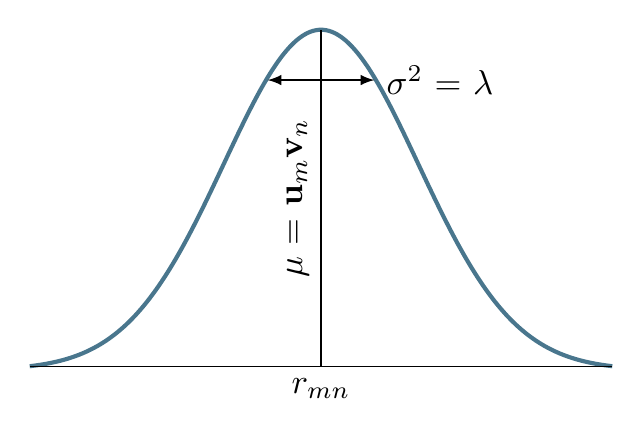
\begin{tikzpicture}[scale=1.25]
    \begin{axis}[
        domain=-3:3,
        samples=200,
        axis lines*=middle,
        xtick=\empty,
        ytick=\empty,
        xlabel=$r_{mn}$,
        ylabel=$\text{$\mu$ = }\vb{u}_m\vb{v}_n$,
        height=5cm,
        width=7.5cm,
        enlargelimits=false,
        clip=false,
        axis on top,
        ]
        \addplot [very thick,cyan!50!black] {exp(-x^2 / 2) / (sqrt(2*pi))};
        \pgfplotsextra{
            \draw [latex-latex] (axis cs:-0.55,0.34) -- (axis cs:0.55,0.34) node [right,right] { $ \sigma^2$ = $\lambda$};
        }
    \end{axis}
    \end{tikzpicture}
    \caption{A diagram of the Gaussian (normal) distribution that describes the predicted rating $r_{mn}$,
    where $\vb{u}_m$ is the trait vector of user $m$, and $\vb{v}_n$ is the trait vector of item $n$.}
    \label{gauss}
\end{figure}

\begin{figure}[h!]
    \centering
    \captionsetup{justification=centering}
    \includegraphics[width=1\textwidth]{graphics/histograms.pdf}
    \caption{Each histogram represent a sample of $1000$ inner products of randomly initialized user vectors ($\vb{u}$) and item vectors ($\vb{v}$).
    The dimensionality of the trait vectors is $k \in \{1, 2, 5, 20\}$} and the value of $\lambda$ is set to $0.1$ for all four histogram plots.
    As you may notice, the value \\of the inner products (predicted ratings) for all four plots are mostly between $0$ and $5$, \\irregardless of the value of $k$.
    \label{hist}
\end{figure}

\newpage

\subsubsection{Embedding in latent space}
The latent space refers to the abstract space that is learned by the recommender system when it is trained using the ALS algorithm.
Ideally, similar users and items should be embedded in the same region of the latent space,
which results in a large inner product of a similar user and item (see Figure~\ref{awe}).
Conversely, dissimiliar users and items should be embedded in different regions of the latent space, 
which results in a small inner product of a dissimilar user and item.

\begin{figure}[h!]
    \centering
    \captionsetup{justification=centering}
    \includegraphics[width=0.7\textwidth]{graphics/awe.png}
    \caption{A diagram of what happens during learning, where similar user vectors and item vectors are 
    embedded in the same direction in the latent space ($k = 2$). \\This diagram was created by Ulrich Paquet~\cite{Ula}.}
    \label{awe}
\end{figure}

\newpage

%%%%%%%%%%%%%%%%%%%%%%%%%%%%%%%%%%%%%%%%%%%%%%%%%%%%%%%%%%%%%%%%%%%%%%%%%%%%%%%%%%%%%%%%%%%%%%%%%%%%%%%%%%%%%%%%%%%%%%%%%%%%%%%%%%%%%%%%%%%%%%

\subsection{ALS: Using only trait vectors}
The alternating least squares (ALS) algorithm is used to obtain the matrix factorization. The ALS algorithm 
iterates between solving for $U$ and $V$ until convergence. More information on the ALS algorithm can be found
\href{}{here}.

The loss function that is used for optimization is the log-likelihood function of all the user and item vectors.
A regularization term is also added for the user and item vectors, where the regularization coefficient is $\tau/2$. 
The regularized log-likelihood function is given by:

\begin{equation} \label{ll1}
    \begin{split}
    \mathcal{L} & = \log{p(R|U,V)} + \log{p(U)} + \log{p(V)} \\
                & = -\dfrac{\lambda}{2} \sum\limits_{mn} (r_{mn} - \vb{u}_{m}^{T} \vb{v}_{n})^2 - \dfrac{\tau}{2} \sum\limits_{m} \vb{u}_{m}^{T} \vb{u}_{m} - \dfrac{\tau}{2} \sum\limits_{n} \vb{v}_{n}^{T} \vb{v}_{n} + \text{const}\text{.}
    \end{split}
\end{equation}

\subsubsection{Update equation for $\vb{u}_{m}$}

The partial derivative of the loss function (Equation \ref{ll1}) with respect to $\vb{u}_{m}$ is written as follows,
where $\Omega(m)$ is the set of movies that user $m$ has rated:

\[
    \dfrac{\partial \mathcal{L}}{\partial \vb{u}_m} 
    = -\lambda \sum\limits_{n \in \Omega(m)} -\vb{v}_{n}(r_{mn} - \vb{u}_{m}^{T} \vb{v}_{n}) - \tau \vb{u}_{m}\text{.}
\]

Setting $\dfrac{\partial \mathcal{L}}{\partial \vb{u}_m}$ equal to zero and rearranging terms leads to

\[
    \Bigg(\lambda \sum\limits_{n \in \Omega(m)} \vb{v}_{n}^{T}\vb{v}_{n} + \tau \vb{I} \Bigg)\vb{u}_m
    = \lambda \sum\limits_{n \in \Omega(m)} \vb{v}_{n} r_{mn}\text{.}
\]

Multiplying both sides of the equation above by the inverse of the matrix on the left-hand side leads to the update equation for $\vb{u}_m$:

\begin{equation} \label{u_1}
    \begin{split}
        \vb{u}_m = \Bigg(\lambda \sum\limits_{n \in \Omega(m)} \vb{v}_{n}^{T}\vb{v}_{n} + \tau \vb{I} \Bigg)^{-1}
        \Bigg(\lambda \sum\limits_{n \in \Omega(m)} \vb{v}_{n} r_{mn}\Bigg)\text{.}
    \end{split}
\end{equation}

\subsubsection{Update equation for $\vb{v}_{n}$}

The partial derivative of the loss function (Equation \ref{ll1}) with respect to $\vb{v}_{n}$ is written as follows,
where $\Psi(n)$ is the set of users that have rated movie $n$:

\[
    \dfrac{\partial \mathcal{L}}{\partial \vb{v}_{n}} = -\lambda \sum\limits_{m \in \Psi(n)} -\vb{u}_{m}(r_{mn} - \vb{u}_{m}^{T} \vb{v}_{n}) - \tau \vb{v}_{n}\text{.}
\]

Setting $\dfrac{\partial \mathcal{L}}{\partial \vb{v}_n}$ equal to zero and rearranging terms:

\[
    \Bigg(\lambda \sum\limits_{m \in \Psi(n)} \vb{u}_{m}^{T}\vb{u}_{m} + \tau \vb{I} \Bigg)\vb{v}_n
    = \lambda \sum\limits_{m \in \Psi(n)} \vb{u}_{m} r_{mn}\text{.}
\]

Multiplying both sides of the equation above by the inverse of the matrix on the left-hand side leads to the update equation for $\vb{v}_n$:

\begin{equation} \label{v_1}
    \begin{split}
        \vb{v}_n = \Bigg(\lambda \sum\limits_{m \in \Psi(n)} \vb{u}_{m}^{T}\vb{u}_{m} + \tau \vb{I} \Bigg)^{-1}
        \Bigg(\lambda \sum\limits_{m \in \Psi(n)} \vb{u}_{m} r_{mn}\Bigg)\text{.}
    \end{split}
\end{equation}

%%%%%%%%%%%%%%%%%%%%%%%%%%%%%%%%%%%%%%%%%%%%%%%%%%%%%%%%%%%%%%%%%%%%%%%%%%%%%%%%%%%%%%%%%%%%%%%%%%%%%%%%%%%%%%%%%%%%%%%%%%%%%%%%%%%%%%%%%%%%%%

\subsection{ALS: Adding bias terms} \label{als_bias}
Now bias terms are added to the likelihood function, one for each user and one for each item.
A regularization term is also added for each bias term, where the regularization coefficient is $-\alpha/2$ 
(and $\alpha$ is a hyperparameter).
The bias terms also need to be updated per iteration.
The regularized log-likelihood function with bias terms included is given by:

\begin{equation} \label{ll2}
    \begin{split}
    \mathcal{L} = & -\dfrac{\lambda}{2} \sum\limits_{mn} \bigg(r_{mn} - (\vb{u}_{m}^{T} \vb{v}_{n} + b_{m}^{(u)} + b_{n}^{(v)})\bigg)^{2} \\
                  & -\dfrac{\tau}{2} \sum\limits_{m} \vb{u}_{m}^{T} \vb{u}_{m} - \dfrac{\tau}{2} \sum\limits_{n} \vb{v}_{n}^{T} \vb{v}_{n} \\
                  & -\dfrac{\alpha}{2} \sum\limits_{m} (b_{m}^{(u)})^{2} - \dfrac{\alpha}{2} \sum\limits_{n} (b_{n}^{(v)})^{2} + \text{const}\text{.}
    \end{split}
\end{equation}

\subsubsection{Update equations for $\vb{u}_{m}$ and $\vb{v}_{n}$}

The update equations for $\vb{u}_m$ and $\vb{v}_n$ with the bias terms is very similar to Equations \ref{u_1} and \ref{v_1}:

\begin{equation}
    \begin{split}
        \vb{u}_m = \Bigg(\lambda \sum\limits_{n \in \Omega(m)} \vb{v}_{n}^{T}\vb{v}_{n} + \tau \vb{I} \Bigg)^{-1}
        \Bigg(\lambda \sum\limits_{n \in \Omega(m)} \vb{v}_{n}(r_{mn} - b_{m}^{(u)} - b_{n}^{(v)})\Bigg)\text{,}
    \end{split}
\end{equation}

\begin{equation}
    \begin{split}
        \vb{v}_n = \Bigg(\lambda \sum\limits_{m \in \Psi(n)} \vb{u}_{m}^{T}\vb{u}_{m} + \tau \vb{I} \Bigg)^{-1}
        \Bigg(\lambda \sum\limits_{m \in \Psi(n)} \vb{u}_{m}(r_{mn} - b_{m}^{(u)} - b_{n}^{(v)})\Bigg)\text{.}
    \end{split}
\end{equation}

\subsubsection{Update equation for $b_{m}^{(u)}$}

The partial derivative of the loss function (Equation \ref{ll2}) with respect to $b_{m}^{(u)}$ is written as:

\[
    \dfrac{\partial \mathcal{L}}{\partial b_{m}^{(u)}} 
    = -\lambda \sum\limits_{n \in \Omega(m)} -(r_{mn} - \vb{u}_{m}^{T} \vb{v}_{n} - b_{m}^{(u)} - b_{n}^{(v)}) - \alpha b_{m}^{(u)}\text{.}
\]

Setting $\dfrac{\partial \mathcal{L}}{\partial b_{m}^{(u)}}$ equal to zero and rearranging terms leads to the update equation for $b_{m}^{(u)}$:

\[
    \alpha b_{m}^{(u)} + \lambda |\Omega(m)| b_{m}^{(u)} = \lambda \sum\limits_{n \in \Omega(m)} (r_{mn} - \vb{u}_{m}^{T} \vb{v}_{n} - b_{n}^{(v)})
\]

\begin{equation}
    \begin{split}
        b_{m}^{(u)} = \dfrac{\lambda}{\alpha + \lambda |\Omega(m)|} \sum\limits_{n \in \Omega(m)} (r_{mn} - \vb{u}_{m}^{T} \vb{v}_{n} - b_{n}^{(v)})\text{.}
    \end{split}
\end{equation}

\subsubsection{Update equation for $b_{n}^{(v)}$}

The partial derivative of the loss function (Equation \ref{ll2}) with respect to $b_{n}^{(v)}$ is written as:

\[
    \dfrac{\partial \mathcal{L}}{\partial b_{n}^{(v)}} 
    = -\lambda \sum\limits_{m \in \Psi(n)} -(r_{mn} - \vb{v}_{n}^{T} \vb{u}_{m} - b_{m}^{(u)} - b_{n}^{(v)}) - \alpha b_{n}^{(v)}\text{.}
\]

Setting $\dfrac{\partial \mathcal{L}}{\partial b_{n}^{(v)}}$ equal to zero and rearranging terms leads to the update equation for $b_{n}^{(v)}$:

\[
    \alpha b_{n}^{(v)} + \lambda |\Psi(n)| b_{n}^{(v)} = \lambda \sum\limits_{m \in \Psi(n)} (r_{mn} - \vb{u}_{m}^{T} \vb{v}_{n} - b_{m}^{(u)})
\]

\begin{equation}
    \begin{split}
       b_{n}^{(v)} = \dfrac{\lambda}{\alpha + \lambda |\Psi(n)|} \sum\limits_{m \in \Psi(n)} (r_{mn} - \vb{u}_{m}^{T} \vb{v}_{n} - b_{m}^{(u)})\text{.}
    \end{split}
\end{equation}


%%%%%%%%%%%%%%%%%%%%%%%%%%%%%%%%%%%%%%%%%%%%%%%%%%%%%%%%%%%%%%%%%%%%%%%%%%%%%%%%%%%%%%%%%%%%%%%%%%%%%%%%%%%%%%%%%%%%%%%%%%%%%%%%%%%%%%%%%%%%%%

\subsection{ALS: Using genre metadata} \label{bruh}
It is possible to use genre metadate for each movie to further expand the log-likelihood function. 
This is done by learning genre trait vectors ($\vb{f}_i$) and modifying the regularizer for the item vectors.
This causes the movies to be embedded into more distinct areas of the latent space, depending on the genres associated
with each movie. A regularization term is introduced for the genre vectors ($\vb{f}_i$), where the regularization 
coefficient is $-\mathcal{B}/2$ (and $\mathcal{B}$ is a hyperparameter). The regularized 
log-likelihood function with biases and genre metadata is written as follows, where $\mathcal{X}(n)$ is the set of
genres that are associated with movie $n$:

\begin{equation} \label{ll3}
    \begin{split}
    \mathcal{L}= & -\dfrac{\lambda}{2} \sum\limits_{mn} \bigg(r_{mn} - (\vb{u}_{m}^{T} \vb{v}_{n} + b_{m}^{(u)} + b_{n}^{(v)})\bigg)^{2} \\
                 & -\dfrac{\tau}{2} \sum\limits_{m} \vb{u}_{m}^{T} \vb{u}_{m} - \dfrac{\tau}{2} \sum\limits_{n} (\vb{v}_{n} - \dfrac{1}{\sqrt{|\mathcal{X}(n)|}}\sum\limits_{i \in \mathcal{X}(n)}\vb{f}_i)^{T} (\vb{v}_{n} - \dfrac{1}{\sqrt{|\mathcal{X}(n)|}}\sum\limits_{i \in \mathcal{X}(n)}\vb{f}_i) \\
                 & -\dfrac{\alpha}{2} \sum\limits_{m} (b_{m}^{(u)})^{2} - \dfrac{\alpha}{2} \sum\limits_{n} (b_{n}^{(v)})^{2} -\dfrac{\mathcal{B}}{2} \sum\limits_{i} \vb{f}_{i}^{T} \vb{f}_{i} + \text{const}\text{.}
    \end{split}
\end{equation}

The update equations for $\vb{u}_m$, $b_{m}^{(u)}$, and $b_{n}^{(v)}$ remain the same as in Section \ref{als_bias}.

\subsubsection{Update equation for $\vb{v}_{n}$}
Using genre metadata changes the update equation for $\vb{v}_{n}$:

\begin{equation}
    \begin{split}
        \vb{v}_n = \Bigg(\lambda \sum\limits_{m \in \Psi(n)} \vb{u}_{m}^{T}\vb{u}_{m} + \tau \vb{I} \Bigg)^{-1}
        \Bigg(\lambda \sum\limits_{m \in \Psi(n)} \vb{u}_{m}(r_{mn} - b_{m}^{(u)} - b_{n}^{(v)}) + \dfrac{\tau}{\sqrt{|\mathcal{X}(n)|}} \sum\limits_{i \in \mathcal{X}(n)} \vb{f}_i\Bigg)\text{.}
    \end{split}
\end{equation}

\subsubsection{Update equation for $\vb{f}_i$}

The partial derivative of the loss function (Equation \ref{ll3}) with respect to $\vb{f}_i$ is written as follows,
where $\mathcal{Z}(i) = {\{n: i \in \mathcal{X}(n)\}}$ (all movies that contain the genre $i$):

\begin{equation}
    \begin{split}
        \dfrac{\partial \mathcal{L}}{\partial \vb{f}_i} &= \tau \Bigg[ \sum\limits_{\mathcal{Z}(i)} \bigg(\vb{v}_{n} - \dfrac{1}{\sqrt{|\mathcal{X}(n)|}} \sum\limits_{j \in \mathcal{X}(n)} \vb{f}_j\bigg) \Bigg] \bigg( \sum\limits_{\mathcal{Z}(i)} \dfrac{1}{\sqrt{|\mathcal{X}(n)|}} \bigg)- \mathcal{B} \vb{f}_i \\
                                                          &= \tau \Bigg[ \sum\limits_{\mathcal{Z}(i)} \bigg(\vb{v}_{n} - \dfrac{1}{\sqrt{|\mathcal{X}(n)|}} \sum\limits_{\{j \in \mathcal{X}(n)\}/i} \vb{f}_j \bigg) 
                                                          - \bigg( \sum\limits_{\mathcal{Z}(i)} \dfrac{1}{\sqrt{|\mathcal{X}(n)|}}\bigg) \vb{f}_i \Bigg]\bigg( \sum\limits_{\mathcal{Z}(i)} \dfrac{1}{\sqrt{|\mathcal{X}(n)|}} \bigg) - \mathcal{B} \vb{f}_i \text{.}
    \end{split}
\end{equation}

Setting $\dfrac{\partial \mathcal{L}}{\partial \vb{f}_i}$ equal to zero and rearranging terms:

\[
    \tau \Bigg(\sum\limits_{\mathcal{Z}(i)}\dfrac{1}{\sqrt{|\mathcal{X}(n)|}}\Bigg)^2 \vb{f}_i + \mathcal{B} \vb{f}_i 
    = \tau \bigg( \sum\limits_{\mathcal{Z}(i)} \dfrac{1}{\sqrt{|\mathcal{X}(n)|}} \bigg) \Bigg[ \sum\limits_{\mathcal{Z}(i)} \bigg( \vb{v}_{n} - \dfrac{1}{\sqrt{|\mathcal{X}(n)|}} \sum\limits_{\{j \in \mathcal{X}(n)\}/i} \vb{f}_j \bigg) \Bigg]\text{.}
\]

Simplifying the equation above yields the update equation for $\vb{f}_i$:

\begin{equation}
    \begin{split}
        \vb{f}_i = \dfrac{\tau \bigg( \sum\limits_{\mathcal{Z}(i)} \dfrac{1}{\sqrt{|\mathcal{X}(n)|}} \bigg)}{\tau \Bigg(\sum\limits_{\mathcal{Z}(i)}\dfrac{1}{\sqrt{|\mathcal{X}(n)|}}\Bigg)^2 + \mathcal{B}} \Bigg[ \sum\limits_{\mathcal{Z}(i)} \bigg( \vb{v}_{n} - \dfrac{1}{\sqrt{|\mathcal{X}(n)|}} \sum\limits_{\{j \in \mathcal{X}(n)\}/i} \vb{f}_j \bigg) \Bigg]\text{.}
    \end{split}
\end{equation}

\newpage

\subsection{Parallelized ALS algorithm}
Yehuda's factorization method is convenient to use, since it is easy to parallelize.
Note that the update equation of one user trait vector is independent from the
update equation of a different user trait vector.
The same holds for the item/genre vector and the bias terms.

This means that the ranges $0, \dots, M$ and $0, \dots, N$ can be split up into the number of CPU cores of the computer
the recommender system is being trained. I implemented multiprocessing with four cores, and the parallel
version of my code executed significantly faster than my unparallelized code.

\section{Evaluation techniques}
The loss function (regularized log-likelihood) should increase monotonically over time. There are also other techniques
to evaluate performance of the model, which are explained in the following subsections.

\subsection{Root mean squared error}
The root mean squared error (RMSE) is computed by averaging the squared errors over all user item pairs, $(m, n) \in \mathcal{R}$:
\begin{equation} \label{rmse}
    \text{RMSE} = \sqrt{\dfrac{1}{\abs{\mathcal{R}}} \sum\limits_{(m, n) \in \mathcal{R}} (\hat{r}_{mn} - {r}_{mn})^2}.
\end{equation}
The RMSE metric is commonly used in machine learning algorthms. Note that there are issues associated with this metric.
Firstly, the RMSE metric tends to emphasize large errors rather than preserving fine neighbourhoods.
Secondly, RMSE tends to emphasize popular items that most users have rated.

\subsection{Mean absolute error}
The mean absolute error (MAE) is computed by averaging the absolute errors over all user item pairs, $(m, n) \in \mathcal{R}$:
\begin{equation} \label{mae}
    \text{MAE} = \dfrac{1}{\abs{\mathcal{R}}} \sum\limits_{(m, n) \in \mathcal{R}} |\hat{r}_{mn} - {r}_{mn}|.
\end{equation}
Unlike the RMSE, the MAE metric does not emphasize large errors. 
However, in machine learning it is less commonly used than the RMSE metric, 
due to the difficulties working with the derivative of the MAE function.

\subsection{Evaluation by inspection}
A simple way to check whether a recommender system is working properly is to see create a ``dummy user'' that has rated a collection of movies.
Now we can use the trained recommender system to predict movies for the dummy user.
Using human intuition, we can argue that if the top recommendations are movies that are similar to the movies that the dummy user has rated highly,
then we assume that the recommender system is working. Conversely, if the recommender system recommends a Horror movie for a 
dummy user that rated a Children movie, then we assume something is wrong with the recommender system. 

Note that while this technique is simple and intuitive, there are several issues associated with this technique, such as:
\begin{itemize}
    \item \textbf{Cold start problem}: Regardless of what the dummy user has rated, the same movies are recommended - usually movies that are very popular (or ``polarizing movies'').
    Fortunately, the use of genre trait vectors in the ALS algorthm mitigates this problem.
    \item \textbf{Outliers}: There could be two movies, with two completely different genres, that are rated by a lot of the same users. This may cause
    unexpected recommendations. This is one of the disadvantages of collaborative filtering, however, the use of genre trait vectors slightly mitigates this problem.
\end{itemize}

\newpage

\section{Parameter tuning}
Due to time constraints, I did not tune any parameters for the recommender system.
The first subsection discusses how I would have tuned the control parameter and hyperparameters, 
and the second subsection discusses what values I selected for the parameters and hyperparameters, 
and also why I selected those values.

\subsection{Parameter tuning using cross-validation}
There is one control parameter, $k$, and four hyperparameters: $\lambda, \tau, \alpha, \beta$.
Parameter tuning is best performed using a random cross-validation search.
Random search can explore a wider range of parameter values and potentially find 
a better set of parameters than with a grid search approach.
To tune the control parameter and four hyperparameters using random cross-validation search:
\begin{enumerate}
    \item Define the range of values for each parameter.
    \item Divide the small/full dataset into a training and validation set.
    \item Define the number of iterations and the number of folds.
    \item For each iteration, select random values for the parameters from their defined ranges.
    \item Train the model with the selected parameter values, and evaluate the performance of the model on the validation set.
    \item Repeat steps $4$ and $5$ for the specified number of iterations and folds.
    \item Select the combination of parameter values that maximizes the performance of the model on the validation set.
\end{enumerate}

\subsection{Choosing parameter values}
Since no parameter tuning was implemented, I chose the value for the control parameter and hyperparameters based on my intuition of the ALS algorithm.
The latent space dimensionality ($k$) is chosen as $20$, recommended by Ulrich Paquet. A value of $k << 20$ will result in a low-dimensional feature representation
of the user and item data, which means the ALS algorithm may underfit the data. A value of $k >> 20$ will cause a non-linear increase in computational
complexity of the ALS algorithm. Since I (regrettably) implemented my recommender system using \texttt{Python},
my computer takes too much time to run the ALS algorithm with a value of $k >> 20$.

The value of $\lambda$ is chosen as $0.1$, and Figure~\ref{hist} is the main reason for this choice. The other hyperparameters, which are
$\tau$, $\alpha$, and $\beta$, are coefficients for the penalty terms of the user, item, and genre trait vectors. I set all three of these hyperparameters
equal to $0.01$. If the value for $\beta$ is decreased, the genre features vectors are less penalized in the loss function, which increases 
the content-based filtering of the recommender system.

The control parameter and hyperparameter values were chosen as follows:
\begin{equation} \label{hp}
    \begin{split}
        k = 20\text{; }\lambda = 0.1\text{; }\tau = 0.01\text{; }\alpha = 0.01\text{; }\beta = 0.01\text{.}
    \end{split}
\end{equation}

\newpage

%%%%%%%%%%%%%%%%%%%%%%%%%%%%%%%%%%%%%%%%%%%%%%%%%%%%%%%%%%%%%%%%%%%%%%%%%%%%%%%%%%%%%%%%%%%%%%%%%%%%%%%%%%%%%%%%%%%%%
%%%%%%%%%%%%%%%%%%%%%%%%%%%%%%%%%%%%%%%%%%%%%%%%%%%%%%%%%%%%%%%%%%%%%%%%%%%%%%%%%%%%%%%%%%%%%%%%%%%%%%%%%%%%%%%%%%%%%
%%%%%%%%%%%%%%%%%%%%%%%%%%%%%%%%%%%%%%%%%%%%%%%%%%%%%%%%%%%%%%%%%%%%%%%%%%%%%%%%%%%%%%%%%%%%%%%%%%%%%%%%%%%%%%%%%%%%%

\section{Experimenal results}
Several different experimental results were gathered by training a model using the ALS algorithm.
In most cases, the models were trained using the ALS update equations described in Section \ref{bruh},
and the values for the control parameter and hyperparameters were selected according to Equation \ref{hp}.

\subsection{Loss and error results}

\subsubsection{Regularized log-likelihood over time}
Figures \ref{r1} and \ref{r2} show the value of the loss function (Equation \ref{ll3}) for 25 iterations of the ALS algorithm.
Note that the value of the loss function is for the training set and is monotonically increasing (since the loss function is negative).

\begin{figure}[h!]
    \centering
    \begin{minipage}{.5\textwidth}
      \centering
      \captionsetup{justification=centering}
      \includegraphics[width=\textwidth]{../src/output/ml-25m/k = 20, ll = 0.1, tau = 0.01, alpha = 0.01, beta = 0.01, iters = 25/loss.pdf}
      \captionof{figure}{Plot of the loss function values over time (using ALS with biases and trait vectors) for the small dataset.}
      \label{r1}
    \end{minipage}%
    \begin{minipage}{.5\textwidth}
      \centering
      \captionsetup{justification=centering}
      \includegraphics[width=\textwidth]{../src/output/ml-25m/k = 20, ll = 0.1, tau = 0.01, alpha = 0.01, beta = 0.01, iters = 25/loss.pdf}
      \captionof{figure}{Plot of the loss function values over time (using ALS with biases and trait vectors) for the full dataset.}
      \label{r2}
    \end{minipage}
\end{figure}

\subsubsection{RMSE and MAE over time}
Figures \ref{r3} and \ref{r4} show the value of the RMSE and MAE (Equations \ref{rmse} and \ref{mae}) for 25 iterations of the ALS algorithm.
Note that ideally both the RMSE and MAE value should decrease over time.

\begin{figure}[h!]
    \centering
    \begin{minipage}{.5\textwidth}
      \centering
      \captionsetup{justification=centering}
      \includegraphics[width=\textwidth]{../src/output/small/k = 20, ll = 0.1, tau = 0.01, alpha = 0.01, beta = 0.01, iters = 25/rmse_mae.pdf}
      \captionof{figure}{Plot of the RMSE and MAE values over time (using ALS with biases and trait vectors) for the small dataset.}
      \label{r3}
    \end{minipage}%
    \begin{minipage}{.5\textwidth}
      \centering
      \captionsetup{justification=centering}
      \includegraphics[width=\textwidth]{../src/output/ml-25m/k = 20, ll = 0.1, tau = 0.01, alpha = 0.01, beta = 0.01, iters = 25/rmse_mae.pdf}
      \captionof{figure}{Plot of the RMSE and MAE values (using ALS with biases and trait vectors) for the full dataset.}
      \label{r4}
    \end{minipage}
\end{figure}

\newpage

\subsection{Two-dimensional trait vector embeddings}

\subsubsection{Item vector embeddings}
Figure \ref{r5} and \ref{r6} show a selection of movies and their two-dimensional embeddings.
For both Figures, the ALS alorithm was run for 10 iterations ($k = 2$), and the hyperparameters are selected as before.
This is done to see whether similar movies are embedded together and opposite movies are embedded in ``opposite''
parts of the space.

For both datasets, the trait vectors in blue indicate that childrens' movies (such as ``Despicable Me'' and ``Shrek'') 
are embedded far away from horror movies (such as ``Saw'' and ``The Conjuring'').

\begin{figure}[h!]
    \centering
    \begin{minipage}{.5\textwidth}
      \centering
      \captionsetup{justification=centering}
      \includegraphics[width=0.8\textwidth]{graphics/small_2D_items.png}
      \captionof{figure}{A scatter plot of the item \\trait vectors for the small dataset.}
      \label{r5}
    \end{minipage}%
    \begin{minipage}{.5\textwidth}
      \centering
      \captionsetup{justification=centering}
      \includegraphics[width=\textwidth]{graphics/full_2D_items.png}
      \captionof{figure}{A scatter plot of the item \\trait vectors for the full dataset.}
      \label{r6}
    \end{minipage}
\end{figure}

\subsubsection{Genre vector embeddings}
Figure \ref{r7} and \ref{r8} the two-dimensional embeddings of the genre trait features.
For both Figures, the ALS alorithm was run for 10 iterations ($k = 2$), and the hyperparameters are selected as before.
This is done to see whether similar genres are embedded together and opposite genres are embedded in ``opposite''
parts of the space.

For both datasets, the genre trait vectors for ``Children'' and ``Horror'' are embedded in opposite parts of the space.
Additionally, the trait vectors for the genres ``Crime'', ``Mystery'', and ``Thriller'' are relatively close to each other,
which makes sense if you think about how movies are categorized by all three of these genres simultaneously.

\begin{figure}[h!]
    \centering
    \begin{minipage}{.5\textwidth}
      \centering
      \captionsetup{justification=centering}
      \includegraphics[width=0.72\textwidth, height=0.6\textwidth]{graphics/small_2D_genre_vectors.pdf}
      \captionof{figure}{A scatter plot of the genre \\trait vectors for the small dataset.}
      \label{r7}
    \end{minipage}%
    \begin{minipage}{.5\textwidth}
      \centering
      \captionsetup{justification=centering}
      \includegraphics[width=0.72\textwidth, height=0.6\textwidth]{graphics/full_2D_genre_vectors.pdf}
      \captionof{figure}{A scatter plot of the genre\\trait vectors for the full dataset.}
      \label{r8}
    \end{minipage}
\end{figure}

\newpage

\subsection{Dummy user predictions}
For this section of results, we set up ``dummy users'' to show that if a the dummy user liked movie X 
(handpicked movie choice) -- the recommendations Y make sense. This is done by creating a user that has rated
one movie 5 stars, updating the user vector and user bias for a number of iterations, 
and returning the ten largest predicted ratings.

\subsubsection{Small dataset results}
The results (Tables \ref{tt1}~-~\ref{tt3}) shown are for three dummy users using the small dataset. The 
results show promise, however the small dataset contains too few movies and user ratings to get desirable recommendations.

The recommendations for the ``Star Wars'' movie are decent, but I would
expect more Star Wars movies to be recommended. 
The recommendations for the ``Lord of the Rings'' movie are the best out of the three,
since the entire Lord of the Rings trilogy is recommended within the top 10 recommendations.
Finally, the recommendations for the ``Toy Story'' movie are the worst, because the system did not
recommend a Toy Story movie and it also only recommended four other animation movies. 

\begin{table}[h!]
    \centering
    \caption{Predictions for Star Wars: Episode II - Attack of the Clones (2002)}
    \label{tt1}
    \resizebox{\textwidth}{!}{%
        \begin{tabular}{|l|l|l|l|}
        \hline
        \textbf{Rank} & \textbf{Movie} & \textbf{Rating} & \textbf{Genres}\\ \hline
            1 & \textbf{Star Wars: Episode II - Attack of the Clones (2002)} & 1.9916 & Action,Adventure,Sci-Fi\\ \hline
            2 & Matrix Revolutions, The (2003) & 1.9446 & Action,Adventure,Sci-Fi,Thriller\\ \hline
            3 & Hellboy (2004) & 1.8965 & Action,Adventure,Fantasy,Horror\\ \hline
            4 & Sgt. Bilko (1996) & 1.8923 & Comedy\\ \hline
            5 & American Pie 2 (2001) & 1.8667 & Comedy\\ \hline
            6 & Oblivion (2013) & 1.8527 & Action,Adventure,Sci-Fi,IMAX\\ \hline
            7 & We Were Soldiers (2002) & 1.8372 & Action,Drama,War\\ \hline
            8 & Saw (2004) & 1.8041 & Horror,Mystery,Thriller\\ \hline
            9 & Click (2006) & 1.7917 & Adventure,Comedy,Drama\\ \hline
            10 & Boys on the Side (1995) & 1.7812 & Comedy,Drama\\ \hline
        \end{tabular}
    }
\end{table}

\begin{table}[h!]
    \centering
    \caption{Predictions for Lord of the Rings: The Return of the King (2003)}
    \label{tt2}
    \resizebox{\textwidth}{!}{%
        \begin{tabular}{|l|l|l|l|}
            \hline
            \textbf{Rank} & \textbf{Title} & \textbf{Score} & \textbf{Genres}\\ \hline
            1 & Old School (2003) & 1.1514 & Comedy\\ \hline
            2 & In the Name of the Father (1993) & 1.1041 & Drama\\ \hline
            3 & \textbf{Lord of the Rings: Two Towers, The (2002)} & 1.1007 & Adventure, Fantasy\\ \hline
            4 & \textbf{Lord of the Rings: Fellowship of the Ring, The (2001)} & 1.0999 & Adventure, Fantasy\\ \hline
            5 & English Patient, The (1996) & 1.0978 & Drama, Romance, War\\ \hline
            6 & Boys Don't Cry (1999) & 1.0780 & Drama\\ \hline
            7 & Willow (1988) & 1.0754 & Action, Adventure, Fantasy\\ \hline
            8 & \textbf{Lord of the Rings: Return of the King, The (2003)} & 1.0752 & Action, Adventure, Drama, Fantasy\\ \hline
            9 & West Side Story (1961) & 1.0709 & Drama, Musical, Romance\\ \hline
            10 & Hellboy (2004) & 1.0420 & Action, Adventure, Fantasy, Horror\\ \hline
        \end{tabular}
    }
\end{table}
    
    
\begin{table}[h!]
    \centering
    \caption{Predictions for Toy Story (1995).}
    \label{tt3}
    \resizebox{\textwidth}{!}{%
        \begin{tabular}{|l|l|l|l|}
            \hline
            \textbf{Rank} & \textbf{Title} & \textbf{Rating} & \textbf{Genres} \\ \hline
            1 & Wild Things (1998) & 1.4163 & Crime, Drama, Mystery, Thriller\\ \hline
            2 & Bend It Like Beckham (2002) & 1.4084 & Comedy, Drama, Romance\\ \hline
            3 & River Runs Through It, A (1992) & 1.3917 & Drama\\ \hline
            4 & Wallace \& Gromit: The Best of Aardman Anim... & 1.3789 & Adventure, Animation, Comedy\\ \hline
            5 & Lost Boys, The (1987) & 1.3717 & Comedy, Horror, Thriller\\ \hline
            6 & Iron Giant, The (1999) & 1.3523 & Adventure, Animation, Children, Drama, Sci-Fi\\ \hline
            7 & Hunchback of Notre Dame, The (1996) & 1.3457 & Animation, Children, Drama, Musical, Romance\\ \hline
            8 & Jackass: The Movie (2002) & 1.3447 & Action, Comedy, Documentary\\ \hline
            9 & Crank (2006) & 1.3264 & Action,Thriller\\ \hline
            10 & Gone with the Wind (1939) & 1.3259 & Drama,Romance,War \\ \hline
            \hline
        \end{tabular}
    }
\end{table}

\newpage

\subsubsection{Full dataset results}
The same three movies was used to create dummy users for the full dataset.
The results for the three dummy users, summarized by Tables \ref{t1}~-~\ref{t3}, are much better and consistent than for the small dataset.

The recommendations for the Star Wars movie are great, with four Star Wars movies in the top $8$ recommendations. 
The recommendations for the Lord of the Rings movie are again the best out of the three movies,
since the Lord of the Rings and ``Hobbit`` trilogies ($6$ movies) are in the top $10$ recommendations.
Finally, the recommendations for the ``Toy Story'' movie are still the worst, with only one Toy Story recommendation.
However, the other recommendations for the Toy Story movie are at least (more or less) the same genre. 

\begin{table}[h!]
    \centering
    \caption{Predictions for Star Wars: Episode II - Attack of the Clones (2002).}
    \label{t1}
    \resizebox{\textwidth}{!}{%
        \begin{tabular}{|l|l|l|l|}
            \hline
            \textbf{Rank} & \textbf{Title} & \textbf{Rating} & \textbf{Genres} \\ \hline
            1 & \textbf{Star Wars: Episode II - Attack of the Clones (2002)} & 5.3498 & Action,Sci-Fi \\ \hline
            2 & \textbf{Star Wars: Episode III - Revenge of the Sith (2005)} & 4.9842 & Action,Sci-Fi \\ \hline
            3 & Naruto Shippuden the Movie: Road to Ninja (2012) & 4.9184 & Action,Adventure,Fantasy \\ \hline
            4 & \textbf{Star Wars: Episode I - The Phantom Menace (1999)} & 4.8043 & Action,Sci-Fi \\ \hline
            5 & 2012: Ice Age (2011) & 4.4698 & Action,Adventure,Sci-Fi \\ \hline
            6 & Dane Cook: Vicious Circle (2006) & 4.0818 & Comedy \\ \hline
            7 & Skins (2017) & 4.0142 & Comedy,Drama \\ \hline
            8 & \textbf{Star Wars: The Clone Wars (2008)} & 3.7469 & Action,Adventure,Animation,Sci-Fi \\ \hline
            9 & Terminal (2004) & 3.5699 & Drama,Thriller \\ \hline
            10 & Kevin Smith: Sold Out - A Threevening with Kevin Smith (2008) & 3.5274 & Comedy \\ \hline
        \end{tabular}
    }
\end{table}
\begin{table}[h!]
    \centering
    \caption{Predictions for Lord of the Rings: The Return of the King (2003).}
    \label{t2}
    \resizebox{\textwidth}{!}{%
        \begin{tabular}{|l|l|l|l|}
            \hline
            \textbf{Rank} & \textbf{Title} & \textbf{Rating} & \textbf{Genres} \\ \hline
            1 & \textbf{Lord of the Rings: The Return of the King, The (2003)} & 4.5797 & Action,Adventure \\ \hline
            2 & \textbf{Lord of the Rings: The Two Towers, The (2002)} & 4.5460 & Adventure,Fantasy \\ \hline
            3 & \textbf{Lord of the Rings: The Fellowship of the Ring, The (2001)} & 4.5226 & Adventure \\ \hline
            4 & The Invisible Guardian (2017) & 4.5072 & Crime,Thriller \\ \hline
            5 & Mute (2018) & 4.4020 & Mystery,Sci-Fi,Thriller \\ \hline
            6 & Queen of Earth (2015) & 4.0153 & Drama \\ \hline
            7 & \textbf{Hobbit: An Unexpected Journey, The (2012)} & 3.9652 & Adventure,Fantasy,IMAX \\ \hline
            8 & Sailor Moon S the Movie: Hearts in Ice (1994) & 3.9606 & Action,Animation,Comedy \\ \hline
            9 & \textbf{The Hobbit: The Battle of the Five Armies (2014)} & 3.9568 & Adventure \\ \hline
            10 & \textbf{Hobbit: The Desolation of Smaug, The (2013)} & 3.9563 & Adventure \\ \hline
        \end{tabular}
    }
\end{table}
\begin{table}[h!]
    \centering
    \caption{Predictions for Toy Story (1995).}
    \label{t3}
    \resizebox{\textwidth}{!}{%
        \begin{tabular}{|l|l|l|l|}
            \hline
            \textbf{Rank} & \textbf{Title} & \textbf{Rating} & \textbf{Genres} \\ \hline
            1 & Son of God (2014) & 5.8015 & Drama \\ \hline
            2 & Atharintiki Daaredi (2013) & 5.7088 & Action,Comedy,Drama \\ \hline
            3 & The Search (1948) & 5.6446 & Drama,War \\ \hline
            4 & The Putin Interviews (2017) & 5.4298 & (no genres listed) \\ \hline
            5 & The Fantastic Flying Books of Mr. Morris Lessmore (2011) & 5.4061 & Children \\ \hline
            6 & Oosaravelli (2011) & 5.2345 & Action,Romance \\ \hline
            7 & Patton Oswalt: Finest Hour (2011) & 5.1999 & Comedy \\ \hline
            8 & \textbf{Toy Story 2 (1999)} & 5.1897 & Adventure,Animation,Children \\ \hline
            9 & Neznaika na lune (1997) & 5.1677 & (no genres listed) \\ \hline
            10 & The Legend of Sleepy Hollow (1949) & 5.0762 & Animation,Comedy,Musical \\ \hline
            \hline
        \end{tabular}
    }
\end{table}

\newpage

\subsection{The most and least polarizing movies}
Note that the magnitude of an item trait vector has an effect on magnitude of the predicted rating for that movie. 
An item vector with a larger magnitude will in some cases lead to a larger inner product with certain user vectors.

Thus, the most polarizing movies are the ones which trait vectors have small magnitudes.
Conversely, the least polarizing movies are the ones which trait vectors have small magnitudes.
The magnitudes of the item trait vectors are calculated using the L1 norm (absolute sum) and the L2 norm (Euclidean norm).

\subsubsection{Small dataset results}
The following Tables (\ref{p1}~-~\ref{p4}) summarizes the most/least polarizing movies in the small dataset using the L1 and L2 norms .

\begin{table}[h!]
    \centering
    \resizebox{0.6\textwidth}{!}{%
        \begin{tabular}{|l|l|}
            \hline
            \textbf{Movies} & \textbf{L1 vector norm}\\ \hline
            Pay It Forward (2000) & 18.5068693\\ \hline
            How to Lose a Guy in 10 Days (2003) & 18.40508315\\ \hline
            Thin Red Line, The (1998) & 17.8846111\\ \hline
        \end{tabular}
    }
    \caption{The three most polarizing movies, using L1 distance.}
    \label{p1}
\end{table}
    
\begin{table}[h!]
    \centering
    \resizebox{0.6\textwidth}{!}{%
        \begin{tabular}{|l|l|}
            \hline
            \textbf{Movies} & \textbf{L1 vector norm}\\ \hline
            Christopher Columbus: The Discovery (1992) & 1.45149368\\ \hline
            Wind and the Lion, The (1975) & 1.49269052\\ \hline
            Fugitive, The (1947) & 1.50684792\\ \hline
        \end{tabular}
    }
    \caption{The three least polarizing movies, using L1 distance.}
    \label{p2}
\end{table}

\begin{table}[h!]
    \centering
    \resizebox{0.6\textwidth}{!}{%
        \begin{tabular}{|l|l|}
            \hline
            \textbf{Movies} & \textbf{L2 vector norm}\\ \hline
            Pay It Forward (2000) & 5.29792418\\ \hline
            Grifters, The (1990) & 4.62169082\\ \hline
            Hellboy (2004) & 4.61594904\\ \hline
        \end{tabular}
    }
    \caption{The three most polarizing movies, using L2 distance.}
    \label{p3}
\end{table}

\begin{table}[h!]
    \centering
    \resizebox{0.6\textwidth}{!}{%
        \begin{tabular}{|l|l|}
            \hline
            \textbf{Movies} & \textbf{L2 vector norm}\\ \hline
            Lilya 4-Ever (Lilja 4-ever) (2002) & 0.42302444\\ \hline
            Hellsinki (Rööperi) (2009) & 0.42750923\\ \hline
            Fugitive, The (1947) & 0.43966882\\ \hline
        \end{tabular}
    }
    \caption{The three least polarizing movies, using L2 distance.}
    \label{p4}
\end{table}

\newpage

\subsubsection{Full dataset results}
The following Tables (\ref{p5}~-~\ref{p8}) summarizes the most/least polarizing movies in the full dataset using the L1 and L2 norms.

\begin{table}[h!]
    \centering
    \resizebox{0.6\textwidth}{!}{%
        \begin{tabular}{|l|l|}
            \hline
            \textbf{Movies} & \textbf{L1 vector norm}\\ \hline
            Birdemic: Shock and Terror (2010) & 40.63732348\\ \hline
            Room, The (2003) & 38.70718889\\ \hline
            Manos: The Hands of Fate (1966) & 34.02765909\\ \hline
        \end{tabular}
    }
    \caption{The three most polarizing movies, using L1 distance.}
    \label{p5}
\end{table}
    
\begin{table}[h!]
    \centering
    \resizebox{0.6\textwidth}{!}{%
        \begin{tabular}{|l|l|}
            \hline
            \textbf{Movies} & \textbf{L1 vector norm}\\ \hline
            64: Part 1 (2016) & 1.67346213\\ \hline 
            64: Part 2 (2016) & 1.68315035\\ \hline
            The Lone Wolf Returns (1935) & 1.68315035\\ \hline
        \end{tabular}
    }
    \caption{The three least polarizing movies, using L1 distance.}
    \label{p6}
\end{table}

\begin{table}[h!]
    \centering
    \resizebox{0.6\textwidth}{!}{%
        \begin{tabular}{|l|l|}
            \hline
            \textbf{Movies} & \textbf{L2 vector norm}\\ \hline
            Room, The (2003) & 11.00425097\\ \hline
            Birdemic: Shock and Terror (2010) & 10.95132207 \\ \hline
            Expelled: No Intelligence Allowed (2008) & 9.21358835 \\ \hline
        \end{tabular}
    }
    \caption{The three most polarizing movies, using L2 distance.}
    \label{p7}
\end{table}

\begin{table}[h!]
    \centering
    \resizebox{0.6\textwidth}{!}{%
        \begin{tabular}{|l|l|}
            \hline
            \textbf{Movies} & \textbf{L2 vector norm}\\ \hline
            64: Part 1 (2016) & 0.45170503 \\ \hline 
            64: Part 2 (2016) & 0.45850453 \\ \hline
            The Lone Wolf Returns (1935) & 0.45850453\\ \hline
        \end{tabular}
    }
    \caption{The three least polarizing movies, using L2 distance.}
    \label{p8}
\end{table}

One result that is particularly interesting to me is that ``The Room'' and ``Birdemic: Shock and Terror''
are the most polarizing movies in the full dataset (both for the L1 and L2 norm). 
The reason why I find this interesting is that both of these movies are seen by the Internet as
bad movies that are ``so bad that it's good'' (i.e. funny to watch). 
Adding to that, I think that if someone has rated on of these two movies it may say a lot about their personality.

\newpage

\section{Conclusion}
This report presents a recommender system using Yehuda's matrix factorization method, which was implemented in \texttt{Python}.

There are several issues with this implementation. Collecting explicit feedback is challenging, since it is typically the case that the
majority of users do not care for rating a movie. Collecting implicit feedback is a much more simple task, so for future work I would
consider implementing a Bayesian personalized ranking~\cite{BPR} (BPR) system. The other issue with the implementation discussed in this report
is that when inferring the trait vectors and the biases it was only a point estimate. The system could by improved by implementing a Variational Bayes~\cite{VB}
solution.

One big issue with my implementation is that I did not use a validation set schema.
This meant that I could not implement cross-validation to properly tune the hyperparameters.
The other issue is that there may be outliers in the data that can cause biased recommendations, and in future work potential outliers will be removed.  

Overall, this implementation manages to handle large and sparse rating matrices. 
Yehuda's matrix factorization method is also relatively easy to implement and can be parallelized for efficient computation on large datasets.

\begin{thebibliography}{}
    \bibitem{Ula} \href{https://ulrichpaquet.com/}{Ulrich Paquet} is the course coordinator and he is referenced for his guidance during this project.
    \bibitem{Yehuda} Koren, Y. (2009). Matrix factorization techniques for recommender systems. Computer, 42(8), 30-37.
    \bibitem{MovieLens} Harper, F. M., \& Konstan, J. A. (2015). The MovieLens Datasets: History and Context. ACM Transactions on Interactive Intelligent Systems (TiiS), 5(4), Article 19. DOI: 10.1145/2827872.
    \bibitem{BPR} Rendle, S., Freudenthaler, C., Gantner, Z., \& Schmidt-Thieme, L. (2009). BPR: Bayesian personalized ranking from implicit feedback. In Proceedings of the Twenty-Fifth Conference on Uncertainty in Artificial Intelligence (UAI'09), (pp. 452-461). AUAI Press.
    \bibitem{VB} Koenigstein, N. and Paquet, U., 2013, October. Xbox movies recommendations: Variational Bayes matrix factorization with embedded feature selection. In Proceedings of the 7th ACM Conference on Recommender Systems (pp. 129-136).
\end{thebibliography}
    
\end{document}